%%=============================================================================
%% Methodologie
%%=============================================================================

\chapter{Methodologie}
\label{ch:methodologie}

%% TODO: Hoe ben je te werk gegaan? Verdeel je onderzoek in grote fasen, en
%% licht in elke fase toe welke stappen je gevolgd hebt. Verantwoord waarom je
%% op deze manier te werk gegaan bent. Je moet kunnen aantonen dat je de best
%% mogelijke manier toegepast hebt om een antwoord te vinden op de
%% onderzoeksvraag.


%section{Studie}

%Voor deze proeven te beginnen, zijn we begonnen met het bestuderen van openvas. De reden hiervoor is dat deze open-source is, en het dus gemakkelijker is om een beeld te krijgen achter de schermen. Nadat de literatuurstudie klaar was, moest er beslist worden hoe het verloop van dit onderzoek zou verlopen. Uitendelijk is er besloten om een gedetailleerd onderzoek te voeren op 


\section{Testen bepalen}

In dit onderzoek zal er met elke scanner 4 scans uitgevoerd worden op elk target. De reden hierachter is dat er in een professionele omgeving 2 punten zijn die belangerijk zijn.Zowel nessus als openvas hebben hiervoor aparte profielen die focussen op een ander deel. Naast deze 2 scans is een credential scan ook een noodzaak om een inzicht te krijgen hoe goed een systeem lokaal beveiligd is (indien men toegang en permissie heeft om deze te scannen met bv. ssh). Voor elke scanner zal er dus een snelle credential, accurate credential, snelle uncredential en een accurate uncredential scan uitgevoerd worden. Dit zal gebeuren in een paar omgevingen die we hieronder bespreken.

Eerst testen we dit op honeypots, dit zijn servers die intentioneel een zwakke configuratie hebben die veel vulnerabilities toont op de scanner. Het doel hiervan is dat deze heel goed opgevolgd moeten worden, en van zodra men activiteit op de server opmerkt dit onderzoeken en kijken of er onbevoegde persoon / malware aanwezig is. Deze test zal bepalen hoeveel vulnerabilities op een zwak systeem gevonden worden voor zowel een linux, als een windows machine.

Hierna zullen de scanners gebruikt worden om een webserver te scannen over het internet. Deze test is een goede weergave voor een deel van een penetration test. We verwachten op de server zelf weinig tot geen fouten, maar de extra informatie die de scanner ons geeft zoals het besturingssysteem of welke diensten er draaien op het systeem. Deze informatie kan gebruikt worden voor andere aanvallen zoals social engineering. Dit is een techniek waarbij een aanvaller zich bijvoorbeeld voordoet als een werknemer van een bedrijf, en op deze manier toegang probeert te krijgen tot het interne systeem. Een ander voorbeeld hiervan is dat een aanvaller een mail kan versturen en zich voordoet als een admin, om zo credentials te krijgen.

\section{Opzetten testomgeving}

Voor dit onderzoek werd er gebruik gemaakt van 4 virtuele machines op Virtualbox versie 5.1.10. Voor de virtuele machines waar er een vulnerability scanner op moest draaien, hebben we gebruik gemaakt van een CentOS minimal image. Deze kregen ook dezelfde instellingen die hieronder vermeld worden:

\begin{itemize}
\item 8000 MB ram
\item 4 CPUs
\item NAT \& host-only interfaces
\end{itemize}

Voor de honeypots gebruikten we een iets minder zware virtuele machine, de instellingen hiervoor worden hieronder ook vermeld. 

\begin{itemize}
\item 1000 MB ram
\item 2 CPUs
\item Host-only interface
\end{itemize}

De fysieke computer waar deze testen op zijn uitgevoerd heeft 16GB ram en een cpu met 4 cores en 8 threads. Tijdens de testen waren er geen andere programmas actief die een impact zouden kunnen hebben op de resultaten. Ook werden alleen de machines die getest moeten worden aangezet zodat beide scanners geen impact op elkaar konden hebben.

\section{Installatie}

\subsection{Nessus}

%WGET COMMANDO BIJZETTEN, NESSUS VERSIE, NESSUS CLI TESTEN
Voor nessus te downloaden op de virtuele machine (met enkel CLI), moeten we naar de productpagina gaan. Sinds we geen extra software op de virtuele machine wouden (zoals FTP of SMB), zullen we wget gebruiken voor de .rpm file te downloaden. Dit is niet zo simpel, sinds de download link een pop up weergeeft voor de juiste versie te kiezen. Na dit probleem op te zoeken, is het duidelijk dat we bepaalde waarden met wget moeten meegeven \textbf{\textit{COMMAND}}.

Na de installatie van de RPM file (38 MB), poort 8834/tcp te openen in firewall-cmd en de service nessusd te starten is de webinterface bereikbaar. Hier moeten we de licentiecode ingeven die we verkregen hebben bij het aanvragen van een nessus home licentie. Hierna volgt een download scherm dat +- 7 minuten duurt. Hierna kunnen we beginnen met scannen.

\subsection{Openvas}

Voor openvas te downloaden op de virtuele machine (met enkel CLI), hebben we 2 opties. We kunnen deze van source compilen, of de \textcite{Openvas-installation}. Wij gebruiken de packages, omdat dit minder tijd in beslag neemt. Voor deze packages te downloaden gebruiken we de atomicorp repository, omdat hiernaar verwezen word op de openvas site.

We installeren de packages voor openvas 9 via yum. De totale grootte van alle packages is 70 MB (185 dependencies). Na deze te downloaden moeten we alles installeren via command line, hiervoor gebruiken we 'openvas-setup'. Deze download eerst alle NVTs (28 MB, verplicht), maar na de download crashed het script omdat we de package 'bzip2' niet geïnstalleerd hebben. We starten het script terug op en merken dat we alle NVTs opnieuw moeten downloaden. Hierna geeft het script een niet fatale error 'certool not found', maar het script gaat verder en blijft vasthangen na 'verify admin password'. Op de achtergrond is het script een databank aan het maken met alle NVTs in, na deze stap is het script gedaan. Het script heeft 23 minuten in beslag genomen.

Na poort 9392/tcp open te zetten in firewall-cmd is het \textit{niet} mogelijk om te connecteren op de webinterface. We gebruiken een ander script 'openvas-check-setup --v9' om te kijken wat er mis is. Deze geeft weer dat de redis server niet gestart is. Deze zit in een failing state, en wil niet herstarten. Na de log files te raadplegen hebben we selinux op 'permissive' gezet, en werkt de redis server nu wel.

Na de check-config nog eens te overlopen, blijkt dat de services van openvas momenteel niet aanstaan. Bij deze opmerkingen staan er tussen haakjes openvassd en openvasmd. Na deze commandos uit te voeren, blijkt de services nog steeds niet te draaien. Na dit verder te onderzoeken, blijkt dat de service openvas-scanner, openvas-manager en gsad noemen. we starten deze op en runnen de check-config opnieuw. 

De config geeft nogmaals een probleem, deze keer omdat de database geen tot weinig gegevens bevat. Hiervoor moeten we het commando 'openvasmd --rebuild' starten. Na 4-5 minuten is deze gedaan en draaien we de check-config nogmaals. Nu geeft deze weer dat er geen SCAP en CERT data aanwezig zijn. Hoewel dit \textit{niet} verplicht is, installeren we deze gegevens voor de volledigheid van de scanner. De sync moet gebeuren met rsync, maar sinds deze sync veel files bevatten die niet groot zijn gaat dit heel traag. Deze duurden samen ongeveer 22 minuten en nemen +-800MB in beslag. 

Als al deze gegevens aanwezig zijn, draaien we het commando check-config nog eens. Deze geeft weer dat selinux moet gedisabled worden. We proberen deze eerst op 'permissive' te zetten, maar het script geeft nog steeds een foutmelding. Na een reboot van de server voor selinux uit te zetten, geeft het script weer dat er een paar packages die \textbf{optioneel} zijn niet aanwezig zijn (zoals alien en net-tools). We installeren deze ook zodat deze geen invloed kunnen hebben op de eindresultaten van de scans.

Uiteindelijk geeft het script weer dat de openvas installatie klaar is voor gebruik. Na het bezoeken van de webinterface blijkt dat dit nog steeds niet mogelijk is. Na te troubleshooten blijkt dat de error in het begin van openvas-setup (certool not found) hier schuldig voor is. Na de package 'gnutls-utils' te installeren en nieuwe certificaten te genereren, is het mogelijk om de webinterface te raadplegen. 

Als we de CLI bekijken, blijkt dat deze niet werkt omdate we niet werken met socket files. We lossen dit op door openvas op localhost te laten luisteren in plaats van een .sock file te gebruiken (openvasmd -a 127.0.0.1), hierna werkt de CLI zoals het hoort.

\subsection{Honeypots}

Voor de linux honeypot hebben we 'metasploitable' genomen. Dit is een linux machine die gebaseerd is op ubuntu 8.04 en een reeks services heeft draaien. Deze services zijn opzettelijk zo zwak mogelijk geconfigureerd zodat men op deze virtuele machines vulnerability scanners kunnen testen en zo leren een penetration test uit te voeren.
% BVV: je bent vrij consequent met het verwijzen naar bronnen (wat super is), waarom dan hier niet? Verwijs in een voetnoot naar de website van metasploitable.
% BVV: 

Voor de windows honeypot hebben we een windows xp machine zonder service packs geïnstalleerd, maar met een aantal servers (SMB,SMTP,SNMP, FTP en IIS). Vooral door deze missende service packs hebben deze veel problemen + er zijn geen opzettelijk slecht geconfigureerde machines zoals metasploitable omdat windows xp onder een licentie valt. 
% BVV: Ik begrijp deze laatste bewering niet...

\subsection{Webservers}

%Als 2de test zullen we een webserver scannen die momenteel in gebruik is door HoGent. \textit{\textbf{*URLS*}}. Hiervoor hebben we een schriftelijke toestemming gekregen door Van Vreckem Bert.


%todo: technische termen uitleggen?
\section{Instellingen scans}

\subsection{Nessus}

% BVV: LET OP: NIET in de eerste persoon schrijven

Nessus heeft in de gratis versie geen profielen voor zowel een snelle scan als een diepe scan. Voor dit onderzoek heb ik voor beide scans zelf een profiel opgesteld. Voor de snelle scan heb ik onderstaande settings gebruikt, deze zorgt dat er een snelle scan geleverd wordt, maar met nog steeds accurate resultaten.

%opzoeken default!
\begin{itemize}
\item alive test = ICMP
\item network type = private LAN
\item port list = default
\item Local port enumerators = SSH,WMI,SNMP
\item port scan technique = SYN
\item Scan web applications (enable generic tests)
\item Scan for malware
\end{itemize}

Voor de diepe scan heb ik een aantal testen aangezet waardoor er een mogelijkheid is dat een bepaalde service stopt met werken. Ook gebruik ik hier een brute-force aanval, waar zwakke gegevens zullen weergegeven worden. De volledige settings ziet u hieronder:

\begin{itemize}
\item alive test = ICMP,TCP, ARP
\item network type = private LAN
\item port list = 0-65535
\item Local port enumerators = SSH,WMI,SNMP, only network port scan when local failed
\item Port scan technique = SYN
\item Search for SSL = all ports
\item Perform thorough tests = yes
\item Test default accounts = yes
\item Scan web applications (enable generic tests)
\begin{itemize}
\item Try all http methods
\item Attempt http parameter pollution
\item Test embedded web servers
\end{itemize}
\item Scan for malware
\item Enable safe checks = no
\end{itemize}

Deze settings zijn zowel voor de windows machine, als de linux machine. Hier is er slechts 1 verschil, namelijk credentials. Voor de linux machine is er een SSH authenticatie, terwijl er voor de windows machine SMB gebruikten. Beide accounts hadden admin / root toegang op het systeem.

\subsection{Openvas}

In tegenstelling tot nessus heeft openvas een reeds voorgemaakte profielen. Voor de snelle scan gebruiken we de 'full and fast' scan methode. Hier worden bijna alle NVTs gebruikt, alleen niet diegene dat ervoor kunnen zorgen dat het systeem onstabiel wordt. Samen met de 'All IANA assigned TCP 2012-02-10' port list (5625 poorten). Dit is een lijst van poorten dat geassocieerd zijn met een 'bekende' service. Dit betekent niet dat dit steeds de service is dat er op draait, maar dient meer als een richtlijn voor een unieke poort te kiezen voor een eigen service. Als alive test hebben we hier voor 'Consider alive' geopteerd, omdat we zeker zijn dat dit systeem zal reageren.

Voor de diepe scan hebben we het profiel 'full and very deep ultimate' genomen. Deze bevat \textit{alle} NVTs (ook diegene dat het systeem onstabiel kunnen maken). Samen met alle TCP poorten (0-65535) en de 'consider alive' optie. Ook hier gebruiken we voor de credential scan SSH voor linux, en SMB voor windows.

Wat ons hier opmerkt is dat openvas standaard voor al zijn voorgemaakte scans een TCP connect scan uitvoert, in tegenstelling tot nessus die standaard SYN gebruikt. SYN is een heel stuk sneller, maar kan onbetrouwbare resultaten geven als het systeem dit als een aanval herkent.

% BVV: Zijn deze profielen equivalent aan de tests in Nessus? Indien niet of indien je dit niet kan bepalen, is de vergelijking dan correct?

\section{Scan resultaten}

In dit deel worden alle resultaten besproken tegenover elk target met elke scanner. Hierbij wordt alleen rekening gehouden met vulnerabilities dat een cvss score hebben van 2 of hoger (dus geen logs). De gevonden vulnerabilities met als rating 'critical' zullen ook kort uitgelegd worden (indien er gelijkaardige resultaten of duplicaten zijn, zal dit vermeld worden). Op het einde zal ik de beide scanners vergelijken op basis van de gevonden vulnerabilities. Deze resultaten worden in het volgende hoofdstuk gebruikt om te controleren of er geen 'false positives' aanwezig zijn. Alle resultaten die hieronder besproken worden zijn getest op 14 Maart, met de nieuwste NVTs die publiek beschikbaar zijn.

\subsection{Nessus}

Voor de credential scans zijn er een aantal opties. Voor de metasploitable credential scan hebben we gekozen voor SSH, omdat dit simpel te gebruiken is, en op bijna alle machines reeds aanwezig is. Voor de windows credential scan hebben we gekozen voor een 'Windows login', hier hebben we een administrator account gegeven waardoor nessus de nodige files kon opvragen.

\subsubsection{Metasploitable: snel zonder credentials}

%todo: een ander soort formaat gebruiken dat minder plek in beslag neemt!
% BVV: en dat het ook makkelijker maakt om te vergelijken. Eventueel begin je met een overzichtstabel en geef je daarna de gedetailleerde resultaten.

\begin{itemize}
\item 6 critical
\item 8 high
\item 36 medium
\item 10 low
\end{itemize}

Deze scan heeft 17 minuten in beslag genomen.

'Debian OpenSSH/OpenSSL Package Random Number Generator Weakness' (CVE-2008-0166): Deze vulnerability komt 2 keer voor en kan ervoor zorgen dat een aanvaller een prompt krijgt via het netwerk, of een man in the middle aanval kan uitvoeren (poort 25 \& 22). Dit zorgt ervoor dat een aanvaller alle data kan lezen die tussen de client en server verstuurd word.

'rexecd Service Detection' (CVE-1999-0618): Rexecd heeft weinig tot geen authenticatie, met geen encryptie. Dit kan gebruikt worden om vanuit het netwerk commandos te versturen naar de host waarop deze draait (poort 512). 

'Rogue Shell Backdoor Detection' (\textbf{geen} CVE): Nessus heeft een poort ontdekt waarop het mogelijk is commandos te versturen met root rechten, zonder enige vorm van authenticatie  (poort 1524).

'Unix Operating System Unsupported Version Detection' (\textbf{geen} CVE): Deze host maakt gebruik van een end of life besturingsysteem (ubuntu 8.04), en krijgt dus geen belangerijke updates meer.

'VNC Server "password" Password' (\textbf{geen} CVE): Men kan inloggen in de VNC server met het wachtwoord 'password'. Hierdoor kan een aanvaller een prompt krijgen (port 5900).

\subsubsection{Metasploitable: snel met credentials}

\begin{itemize}
\item 8 critical
\item 7 high
\item 29 medium
\item 10 low
\end{itemize}

Deze scan heeft 11 minuten in beslag genomen. Dit is 6 minuten minder als de scan zonder credentials. Dit is te verklaren door het feit dat nessus om netwerk gebruik en tijd te besparen, het commando 'netstat' uitvoert. Hierdoor kan nessus alle poorten zien die openstaan, en op basis hiervan de scan verder uitvoeren. Hieronder zijn de extra vulnerabilities die nessus ontdekt heeft met de credential scan.

'Bash Remote Code Execution (Shellshock)' (CVE-2014-6271 \& CVE-2014-7169): Een zeer ernstige bug (vergelijkbaar met de meer recentere \textit{heartbleed} bug) dat ervoor zorgt dat een aanvaller toegang krijgt tot een machine, dit kwam door de manier waarop bash funcites afhandelt. De gevolgen van deze bug zijn reeds besproken in het deel \textit{inleiding - requirements}.

'Weak Debian OpenSSH Keys in \textasciitilde/.ssh/authorized\_keys' (CVE-2008-0166): Er is een zwakke ssh key aanwezig in de authorized\_keys file. Hierdoor kan een aanvaller een brute-force aanval gebruiken om toegang te krijgen tot het systeem. Een brute-force aanval is (in de meeste gevallen) een aanvaller die met behulp van een programma een lijst van wachtwoorden afgaat in de hoop dat deze toegang krijgt tot een account, maar in dit geval gaat het over een 'exhaustive key search'. Hier zal een aanvaller in plaats van zich op het wachtwoord te richten proberen de 'key' te raden, waardoor hij het gewone wachtwoord van de gebruiken kan achterhalen.

%todo: opzoeken waarom niet?
Zoals u hierboven kunt zien zijn er 3 unieke vulnerabilities toegevoegd, terwijl er maar 2 resultaten meer zijn. De vulnerability van ubuntu end of life wordt niet meer weergegeven.

\subsubsection{Metasploitable: diep zonder credentials}

\begin{itemize}
\item 6 critical
\item 10 high
\item 40 medium
\item 10 low
\end{itemize}

Deze scan heeft 42 minuten geduurt, en heeft geen extra critical vulnerabilities opgeleverd. De extra 2 high vulnerabilities zijn een SQL injectie, en een command execution. Deze zijn dus beiden gerelateerd aan de extra web server scans.

\subsubsection{Metasploitable: diep met credentials}

\begin{itemize}
\item 9 critical
\item 10 high
\item 38 medium
\item 8 low
\end{itemize}

Deze scan heeft  44 minuten geduurt, en heeft slechts 1 extra vulnerability extra gegeven. Deze is een extra verzameling van CVE's over shellshock (CVE-2014-6277 \& CVE-2014-6278).

\subsubsection{Windows: snel zonder credentials}

\begin{itemize}
\item 17 critical
\item 5 high
\item 10 medium
\item 3 low
\end{itemize}

Deze scan heeft 3 (!) minuten geduurt.

'ASN.1 Multiple Integer Overflows (SMTP check)' (CVE-2003-0818): Hierdoor kan een aanvaller code uitvoeren op een systeem. Hiervoor moet men een speciaal SMTP authenticate packet versturen.

'Microsoft IIS 6.0 \& Windows XP Unsupported Version Detection' (\textbf{geen} CVE): End of life voor de webserver en het besturingssysteem, op zich is dit geen vulnerability. Deze informatie kan wel gebruikt worden om andere vulnerabilities te vinden.

' Cumulative Update for Microsoft RPC/DCOM' (CVE-2003-0352 \& CVE-2003-0715 \& CVE-2003-0528 \& CVE-2003-0605 \& CVE-2003-0813 \& CVE-2004-0116 \& CVE-2003-0807 \& CVE-2004-0124 \& CVE-2008-4250): Dit is een reeks van vulnerabilities die een reeks patches nodig hadden om volledig opgelost te kunnen geraken, hierdoor zijn er een reeks verschillende CVE nummers. Deze exploit maakt het mogelijk voor een aanvaller om code uitvoeren met systeem rechten. Deze vulnerability reeks werd gebruikt om een aantal worms te verspreiden zoals blaster en lovesan.

'ASN.1 Vulnerability Could Allow Code Execution' (CVE-2003-0818): Deze vulnerability zorgt ervoor dat een aanvaller code kan uitvoeren op het systeem, door een speciaal NTLM (een reeks protocollen dat instaat voor de veiligheid van ingelogde gebruikers) packet te versturen.

'Security Update for Microsoft Windows' (CVE-2003-0533): Een bug in LSASS (het deel van windows dat zorgt voor de beveiliging, en het aanmaken van accounts) zorgt ervoor dat een aanvaller commandos kan uitvoeren met systeem rechten.

'Microsoft Windows Task Scheduler Remote Overflow' (CVE-2004-0212): Nogmaals een exploit om op afstand code te kunnen uitvoeren op een machine. Deze keer door een bug in de 'Task scheduler' van windows.

'Vulnerability in SMB Could Allow Remote Code Execution (CVE-2005-1206 \& CVE-2008-4834 \& CVE-2008-4835 \& CVE-2008-4114): Deze vulnerability komt 2 keer voor. Een aanvaller kan (zonder the authenticeren) code uitvoeren door een bug in het SMB protocol. Hieronder volgt nog een 'speciale' SMB vulnerability waar meer uitleg nodig is.

'ETERNALBLUE, ETERNALCHAMPION, ETERNALROMANCE, and ETERNALSYNERGY SMB vulnerabilities' (CVE-2017-0143 \& CVE-2017-0144 \& CVE-2017-0145 \& CVE-2017-0146 \& CVE-2017-0147 \& CVE-2017-0148): Deze reeks vulnerabilities zijn reeds onlangs aan het licht gekomen. Ze worden actief misbruikt op het internet door de 'wannacry' worm en de verschillende varianten. Deze bug (die gevonden werd door NSA, maar niet gedeeld werd met microsoft) heeft voor een ongeziene verspreiding van de cryptolocker gezorgd. Hiermee is het mogelijk om code op een systeem uit te voeren, en verschillende malware programma's op de host te downloaden. 

'Vulnerability in Printer Spooler Service Could Allow Remote Code Execution' (CVE-2005-1984): Door deze bug kan een aanvaller de spooler service laten crashen, of in het ergste geval code uitvoeren op het systeem.

%TODO: msdtc uitleggen?
'Vulnerabilities in MSDTC Could Allow Remote Code Execution' (CVE-2005-2119 \& CVE-2005-1978 \& CVE-2005-1979 \& CVE-2005-1980 \& CVE-2006-0034 \& CVE-2006-1184): Deze exploit komt 2 keer voor. Door een vulnerability in de MSDTC kan een aanvaller verschillende exploits toepassen (bv. local privilege escalation waarbij een reeds ingelogde gebruiker toegang krijgt tot meer permissies).
 
\subsubsection{Windows: snel met credentials}

\begin{itemize}
\item 18 critical
\item 5 high
\item 8 medium
\item 3 low
\end{itemize}

Deze scan heeft 2 (!) minuten geduurt.

Het enige verschil (voor de critical vulnerabilities) is 'MS03-043: Buffer Overrun in Messenger Service (CVE-2003-0717)'. Hoewel deze in dezelfde patch wordt opgelost als de printer spooler service, heeft de uncredential scan deze niet gedetecteerd. De andere vulnerabilities komen overeen.

\subsubsection{Windows: diep zonder credentials}

\begin{itemize}
\item 18 critical
\item 5 high
\item 10 medium
\item 3 low
\end{itemize}

Deze scan heeft 8 minuten geduurt, en bevat geen veranderingen ten opzichte van de vorige scan.

\subsubsection{Windows: diep met credentials}

\begin{itemize}
\item 18 critical
\item 5 high
\item 10 medium
\item 3 low
\end{itemize}

Deze scan heeft 10 minuten geduurt, en bevat geen veranderingen ten opzichte van de vorige scan.

%todo: kijken of nessus & openvas iets zeggen als credentials fout zijn
%todo: openvas --> cvss v2, nesuss cvss v?
%todo: vergelijken welke overeenkomen enzo
\subsection{Openvas}

Ook voor openvas hebben we SSH gekozen voor de metasploitable credential scan, maar voor windows is dit ingewikkelder. Hier moeten we een SMB user geven, maar na het testen hiervan waren er geen verschillen tussen de credential en non-credential scans. 

Openvas gaf geen error terug dat de credentials niet juist waren, maar na onderzoek blijkt dat men eerst een uitvoerbaar bestand (.exe) moet downloaden via openvas, deze op de machine die je wilt scannnen te openen zodat de gebruiker aangemaakt wordt. Na deze stappen te ondernemen was er nog steeds geen verschil tussen de 2 scans. Voor openvas moet ook de optie 'easy file sharing' niet aanstaan (enkel op windows XP machines). Hierna gaf de scanner een opmerkelijk aantal resultaten meer ten opzichte van de non-credential.

\subsubsection{Metasploitable: snel zonder credentials}

\begin{itemize}
\item 24 high
\item 42 medium
\item 4 low
\end{itemize}

%todo: deze blok tekst verplaatsen?
Deze scan heeft 18 minuten geduurt. Wat hier opvallend is, is dat er geen rekening met de 'critical' categorie gehouden werd. Dit duid op het gebruik van cvss versie 2 dat nog geen critical categorie had. Deze versie heeft een compleet andere formule voor het bekomen van het resultaat, en zorgt ervoor dat deze moeilijker te vergelijken zijn met de 3de versie die in 2015 in gebruik genomen werd.

\subsubsection{Metasploitable: snel met credentials}

\begin{itemize}
\item 121 high
\item 161 medium
\item 14 low
\end{itemize}

Deze scan duurde 19 minuten.

\subsubsection{Metasploitable: diep zonder credentials}

\begin{itemize}
\item 27 high
\item 44 medium
\item 4 low
\end{itemize}

Deze scan duurde 37 minuten.

\subsubsection{Metasploitable: diep met credentials}

\begin{itemize}
\item 124 high
\item 165 medium
\item 14 low
\end{itemize}

Deze scan duurde 39 minuten.

\subsubsection{Windows: snel zonder credentials}

\begin{itemize}
\item 7 high
\item 11 medium
\item 0 low
\end{itemize}

Deze scan duurde 11 minuten.

\subsubsection{Windows: snel met credentials}

\begin{itemize}
\item 252 high
\item 56 medium
\item 2 low
\end{itemize}

Deze scan duurde 14 minuten.

\subsubsection{Windows: diep zonder credentials}

\begin{itemize}
\item 9 high
\item 12 medium
\item 0 low
\end{itemize}

Deze scan duurde 21 minuten. Terwijl de scanner bezig was, is er op de windows xp machiene de volgende boodschap verschenen: 


\begin{figure}[h]
\caption{Windows xp crash}
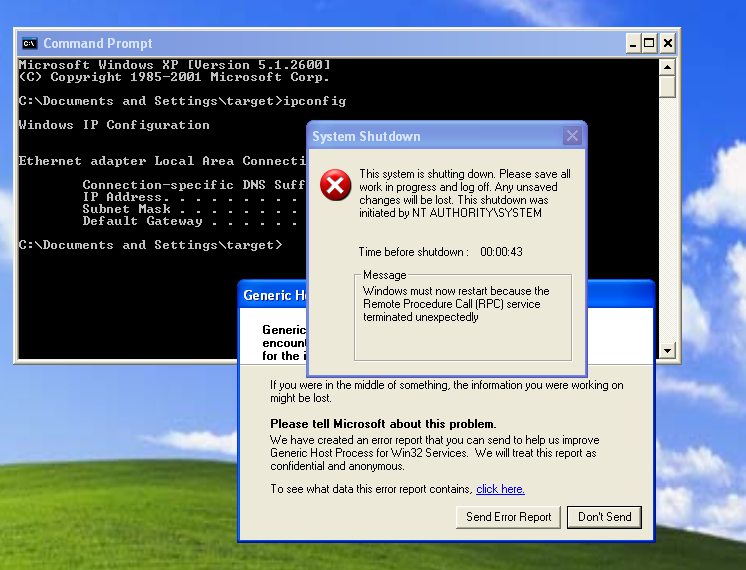
\includegraphics[width=10.0cm]{img/openvas-full.png}
\end{figure}


Hierdoor moest het systeem herstarten. Op het einde van deze scan als de machine herstart was, was het niet mogelijk om een actie uit te voeren hierop. Het besturingssysteem reageerde compleet niet meer, en moest dus opnieuw herstart worden.

\subsubsection{Windows: diep met credentials}

\begin{itemize}
\item 254 high
\item 57 medium
\item 2 low
\end{itemize}

Deze scan duurde 25 minuten. Ook hier deed het scenario van de vorige test zich voor (2 keer herstarten).

\subsection{Resultaat}

\section{Scan resultaten valideren}

Een scanner kan veel vulnerabilities tonen, maar als meer dan de helft van de resultaten false positives zijn, heeft het geen nut om een scan uit te voeren. Hoewel 'false positives' zeker een probleem zijn, is er een groter probleem dat niet direct opvalt. Dit wordt mooi samengevat met de quote: "The real problem is not false positives, it's false negatives", hiermee bedoelt men dat het niet erg is als een scanner soms eens een false positive geeft, zolang hij geen echt vulnerabilities negeert.

Helaas is er geen compelete lijst van vulnerabilities voor zowel windows xp als metasploitable. Een reden hiervoor is dat men constant nieuwe vulnerabilities vind, hierdoor zou de lijst na een aantal maanden of jaren niet meer relevant zijn. Ook de methode die gebruikt werd in voorgaande onderzoeken (met behulp van autopwn in metasploit), bestaat momenteel niet meer. Hierbij is er nog een extra uitdaging omdat nessus met cvss verise 3 werkt, terwijl openvas nog steeds versie 2 gebruikt. Dit kan ervoor zorgen dat de score die een vulnerability krijgt zeer drastisch veranderd. 

Een voorbeeld hiervan is de windows xp machine. Nessus geeft een 'low' resultaat omdat er een X server edetecteerd werd, terwijl dit bij openvas een 'high' vulnerability is. Om toch enige methode van filter te gebruiken, zullen we alle 'critical' vulnerabilities van nessus en de vulnerabilities met een score van 10 tot 9 in openvas onderzoeken. 

Hiervoor zullen we vergelijken of een vulnerability van 1 scanner te vinden is in de andere scanner (zonder rekening te houden met de cvss score). Op deze manier kunnen we nakijken dat de scanners dezelfde vulnerabilities ontdekken, ondanks de verschillende cvss versies. Indien er een vulnerability is dat slechts door 1 scanner wordt ontdekt, zullen we onderzoeken of dit niet over een 'false positive' gaat.


\section{Analyseren van de data}

%alle gevonden data in een tabel gieten, voor en nadelen nog is opsommen en \textit{persoonlijke mening geven?}

% BVV: Geen *persoonlijke mening* geven, enkel staalharde feiten en cijfers waar niet over gediscussieerd kan worden...